\let\negmedspace\undefined
\let\negthickspace\undefined
\documentclass[journal,12pt,twocolumn]{IEEEtran}
\usepackage{cite}
\usepackage{amsmath,amssymb,amsfonts,amsthm}
\usepackage{algorithmic}
\usepackage{graphicx}
\usepackage{textcomp}
\usepackage{xcolor}
\usepackage{txfonts}
\usepackage{listings}
\usepackage{enumitem}
\usepackage{mathtools}
\usepackage{gensymb}
\usepackage[breaklinks=true]{hyperref}
\usepackage{tkz-euclide} % loads  TikZ and tkz-base
\usepackage{listings}
\usepackage{gvv}
%
%\usepackage{setspace}
%\usepackage{gensymb}
%\doublespacing
%\singlespacing

%\usepackage{graphicx}
%\usepackage{amssymb}
%\usepackage{relsize}
%\usepackage[cmex10]{amsmath}
%\usepackage{amsthm}
%\interdisplaylinepenalty=2500
%\savesymbol{iint}
%\usepackage{txfonts}
%\restoresymbol{TXF}{iint}
%\usepackage{wasysym}
%\usepackage{amsthm}
%\usepackage{iithtlc}
%\usepackage{mathrsfs}
%\usepackage{txfonts}
%\usepackage{stfloats}
%\usepackage{bm}
%\usepackage{cite}
%\usepackage{cases}
%\usepackage{subfig}
%\usepackage{xtab}
%\usepackage{longtable}
%\usepackage{multirow}
%\usepackage{algorithm}
%\usepackage{algpseudocode}
%\usepackage{enumitem}
%\usepackage{mathtools}
%\usepackage{tikz}
%\usepackage{circuitikz}
%\usepackage{verbatim}
%\usepackage{tfrupee}
%\usepackage{stmaryrd}
%\usetkzobj{all}
%    \usepackage{color}                                            %%
%    \usepackage{array}                                            %%
%    \usepackage{longtable}                                        %%
%    \usepackage{calc}                                             %%
%    \usepackage{multirow}                                         %%
%    \usepackage{hhline}                                           %%
%    \usepackage{ifthen}                                           %%
  %optionally \brak{for landscape tables embedded in another document}: %%
%    \usepackage{lscape}     
%\usepackage{multicol}
%\usepackage{chngcntr}
%\usepackage{enumerate}

%\usepackage{wasysym}
%\documentclass[conference]{IEEEtran}
%\IEEEoverridecommandlockouts
% The preceding line is only needed to identify funding in the first footnote. If that is unneeded, please comment it out.

\newtheorem{theorem}{Theorem}[section]
\newtheorem{problem}{Problem}
\newtheorem{proposition}{Proposition}[section]
\newtheorem{lemma}{Lemma}[section]
\newtheorem{corollary}[theorem]{Corollary}
\newtheorem{example}{Example}[section]
\newtheorem{definition}[problem]{Definition}
%\newtheorem{thm}{Theorem}[section] 
%\newtheorem{defn}[thm]{Definition}
%\newtheorem{algorithm}{Algorithm}[section]
%\newtheorem{cor}{Corollary}
\newcommand{\BEQA}{\begin{eqnarray}}
\newcommand{\EEQA}{\end{eqnarray}}
\newcommand{\define}{\stackrel{\triangle}{=}}
\theoremstyle{remark}
\newtheorem{rem}{Remark}

%\bibliographystyle{ieeetr}
\begin{document}
%

\bibliographystyle{IEEEtran}


\vspace{3cm}

\title{
%  \logo{
Assignment-1 

\large{EE:1205 \brak{Signals  Systems}}

Indian Institute of Technology, Hyderabad
%  }
}
\author{Md Ayaan Ashraf

EE23BTECH11041
}  
%\title{
%  \logo{Matrix Analysis through Octave}{\begin{center}\includegraphics[scale=.24]{tlc}\end{center}}{}{HAMDSP}
%}


% paper title
% can use linebreaks \\ within to get better formatting as desired
%\title{Matrix Analysis through Octave}
%
%
% author names and IEEE memberships
% note positions of commas and nonbreaking spaces \brak{ ~ } LaTeX will not break
% a structure at a ~ so this keeps an author's name from being broken across
% two lines.
% use \thanks{} to gain access to the first footnote area
% a separate \thanks must be used for each paragraph as LaTeX2e's \thanks
% was not built to handle multiple paragraphs
%
%\author{<-this % stops a space
%\thanks{}}
%}
% note the % following the last \IEEEmembership and also \thanks - 
% these prevent an unwanted space from occurring between the last author name
% and the end of the author line. i.e., if you had this:
% 
% \author{....lastname \thanks{...} \thanks{...} }
%                     ^------------^------------^----Do not want these spaces!
%
% a space would be appended to the last name and could cause every name on that
% line to be shifted left slightly. This is one of those "LaTeX things". For
% instance, "\textbf{A} \textbf{B}" will typeset as "A B" not "AB". To get
% "AB" then you have to do: "\textbf{A}\textbf{B}"
% \thanks is no different in this regard, so shield the last } of each \thanks
% that ends a line with a % and do not let a space in before the next \thanks.
% Spaces after \IEEEmembership other than the last one are OK \brak{and needed} as
% you are supposed to have spaces between the names. For what it is worth,
% this is a minor point as most people would not even notice if the said evil
% space somehow managed to creep in.



% The paper headers
%\markboth{Journal of \LaTeX\ Class Files,~Vol.~6, No.~1, January~2007}%
%{Shell \MakeLowercase{\textit{et al.}}: Bare Demo of IEEEtran.cls for Journals}
% The only time the second header will appear is for the odd numbered pages
% after the title page when using the twoside option.
% 
% *** Note that you probably will NOT want to include the author's ***
% *** name in the headers of peer review papers.                   ***
% You can use \ifCLASSOPTIONpeerreview for conditional compilation here if
% you desire.




% If you want to put a publisher's ID mark on the page you can do it like
% this:
%\IEEEpubid{0000--0000/00\$00.00~\copyright~2007 IEEE}
% Remember, if you use this you must call \IEEEpubidadjcol in the second
% column for its text to clear the IEEEpubid mark.



% make the title area
\maketitle

\newpage

%\tableofcontents

\bigskip
 
\renewcommand{\thefigure}{\theenumi}
\renewcommand{\thetable}{\theenumi}
%\renewcommand{\theequation}{\theenumi}
\section*{\textit{\textbf{Question 10.5.3.12:}}}
 Find the sum of the first 40 positive integers divisible by 6.
\section*{\textit{\textbf{Solution:}}}

\begin{table}[ht]
  \centering
  \begin{tabular}{|c||c||c|}
    \hline
    Parameter & Description & Value \\
    \hline
     x(0) & First Term & 6\\
     \hline
     d & Common Difference & 6\\
    \hline
  \end{tabular}
  \vspace{2mm}
  \caption{Parameter Table 10.5.3.12}
\end{table}


\begin{align}
x\brak{n}= &\brak{6+6n}u\brak{n}\\
\implies X\brak{z}= &\frac {x\brak{0}} {\brak{1-z^{-1}}} + \frac {dz^{-1}} {\brak{1-z^{-1}}^2} \\
= &\frac6{1-z^{-1}} + \frac{6z^{-1}}{\brak{1-z^{-1}}^{2}}\\
\implies X\brak{z}=& \frac6{{\brak{1-z^{-1}}}^2} ,\quad |z|>1\\
y\brak{n}=& x\brak{n}* u\brak{n}\\
\implies Y\brak{z}=& X\brak{z}U\brak{z} \\
= & \frac6{{\brak{1-z^{-1}}}^2}\frac1 {\brak{1-z^{-1}}} \\
=& \frac{6}{\brak{1-z^{-1}}^{3}}, \quad |z|>1
\end{align}
Using contour integration to find the inverse Z-transform:\\
\begin{align}
    \implies y\brak{39}=&\dfrac{1}{2\pi j}\oint_{C}Y\brak{z} \;z^{38} \;dz\\
    =&\dfrac{1}{2\pi j}\oint_{C}\dfrac{6z^{38}}{\brak{{1-z^{-1}}}^{3}} \;dz 
\end{align}
We can observe that there is only a three times repeated pole at z=1,
\begin{align}
    \implies R&=\dfrac{1}{\brak {m-1}!}\lim\limits_{z\to a}\dfrac{d^{m-1}}{dz^{m-1}}\brak {{\brak{z-a}}^{m}f\brak z}  
\end{align}
\begin{align}
    &=\dfrac{1}{\brak {2}!}\lim\limits_{z\to 1}\dfrac{d^{2}}{dz^{2}}\brak {{\brak{z-1}}^{3}\dfrac{6z^{41}}{{\brak{z-1}}^3}}   \\
    &=3\lim\limits_{z\to 1}\dfrac{d^2}{dz^2}\brak{z^{41}}\\
    &=4920
\end{align}
\begin{align}
    \therefore \boxed{y\brak{39}=4920}
\end{align}
\begin{figure}[ht]
    \centering
    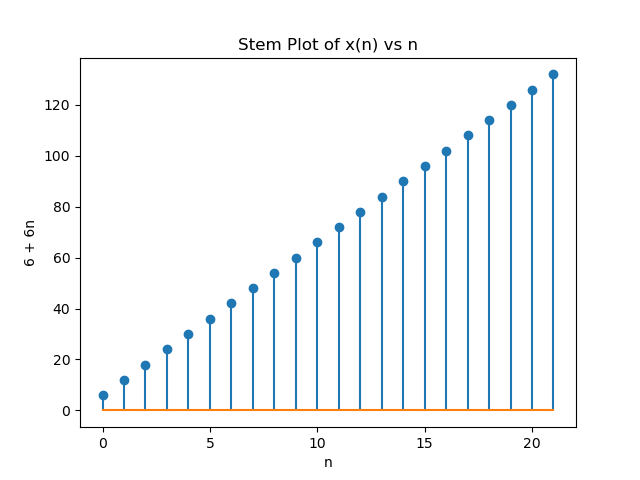
\includegraphics[width=\columnwidth]{figs/fig1.png}
    \caption{Plot of x\brak{n} $vs$ n}
    \label{fig: 10.5.3.12}
\end{figure}
\end{document}
